\documentclass[12pt]{article}
\usepackage{setspace}
\setlength{\parindent}{4em}
\usepackage{fancyvrb}
\usepackage{graphicx}
\usepackage{geometry}
\renewcommand\thesection{\arabic{section}}
\renewcommand\thesubsection{\thesection.\arabic{subsection}}
\geometry{letterpaper, portrait, margin=1in}

%%%Title Page%%%
\title{\vspace{3cm}Lab 03\bigbreak Designing the Toy Processor Datapath}
\author{
{\normalsize
\begin{tabular}{l r r}
 & \textbf{Ryan Cruz} & \textbf{Zachary Davis}\\
\textbf{Category} & ryan.cruz25@uga.edu & zachdav@uga.edu\\
\hline
Pre-lab 						  & 50 & 50\\
In-lab Module \& Testbench Design & 50 & 50\\
In-lab Testbench Sim. \& Analysis & 50 & 50\\
In-lab FPGA Synthesis \& Analysis & 50 & 50\\
Lab Report Writing 				  & 50 & 50\\
\end{tabular}
}}
%%%%%%%%%%%%%%%%%

\begin{document}
\maketitle
\newpage
\setstretch{2.5} % for custom spacing
\tableofcontents
\setstretch{1} % for custom spacing
\newpage

\section{Lab Purpose} \vspace{-.7cm} \line(1,0){470}
	\paragraph{} The purpose of this lab is to create a 4-bit ALU using the schematic method in Xilinx. This will be our first full project that involves creating multiple schematic modules that will eventually be compiled to create a top module that can be implemented on the board. We will design the basic parts of an ALU, including an adder/subtractor, a logic extender, an arithmetic extender, and eventually piece it all together with a UCF and seven segment display driver that will allow us to use this on the board.
				
\section{Implementation Details} \vspace{-.7cm} \line(1,0){470}
	\subsection{Part 0}
		We began by building a full adder, the first basic component of the ALU.
		
%		\begin{center}
%			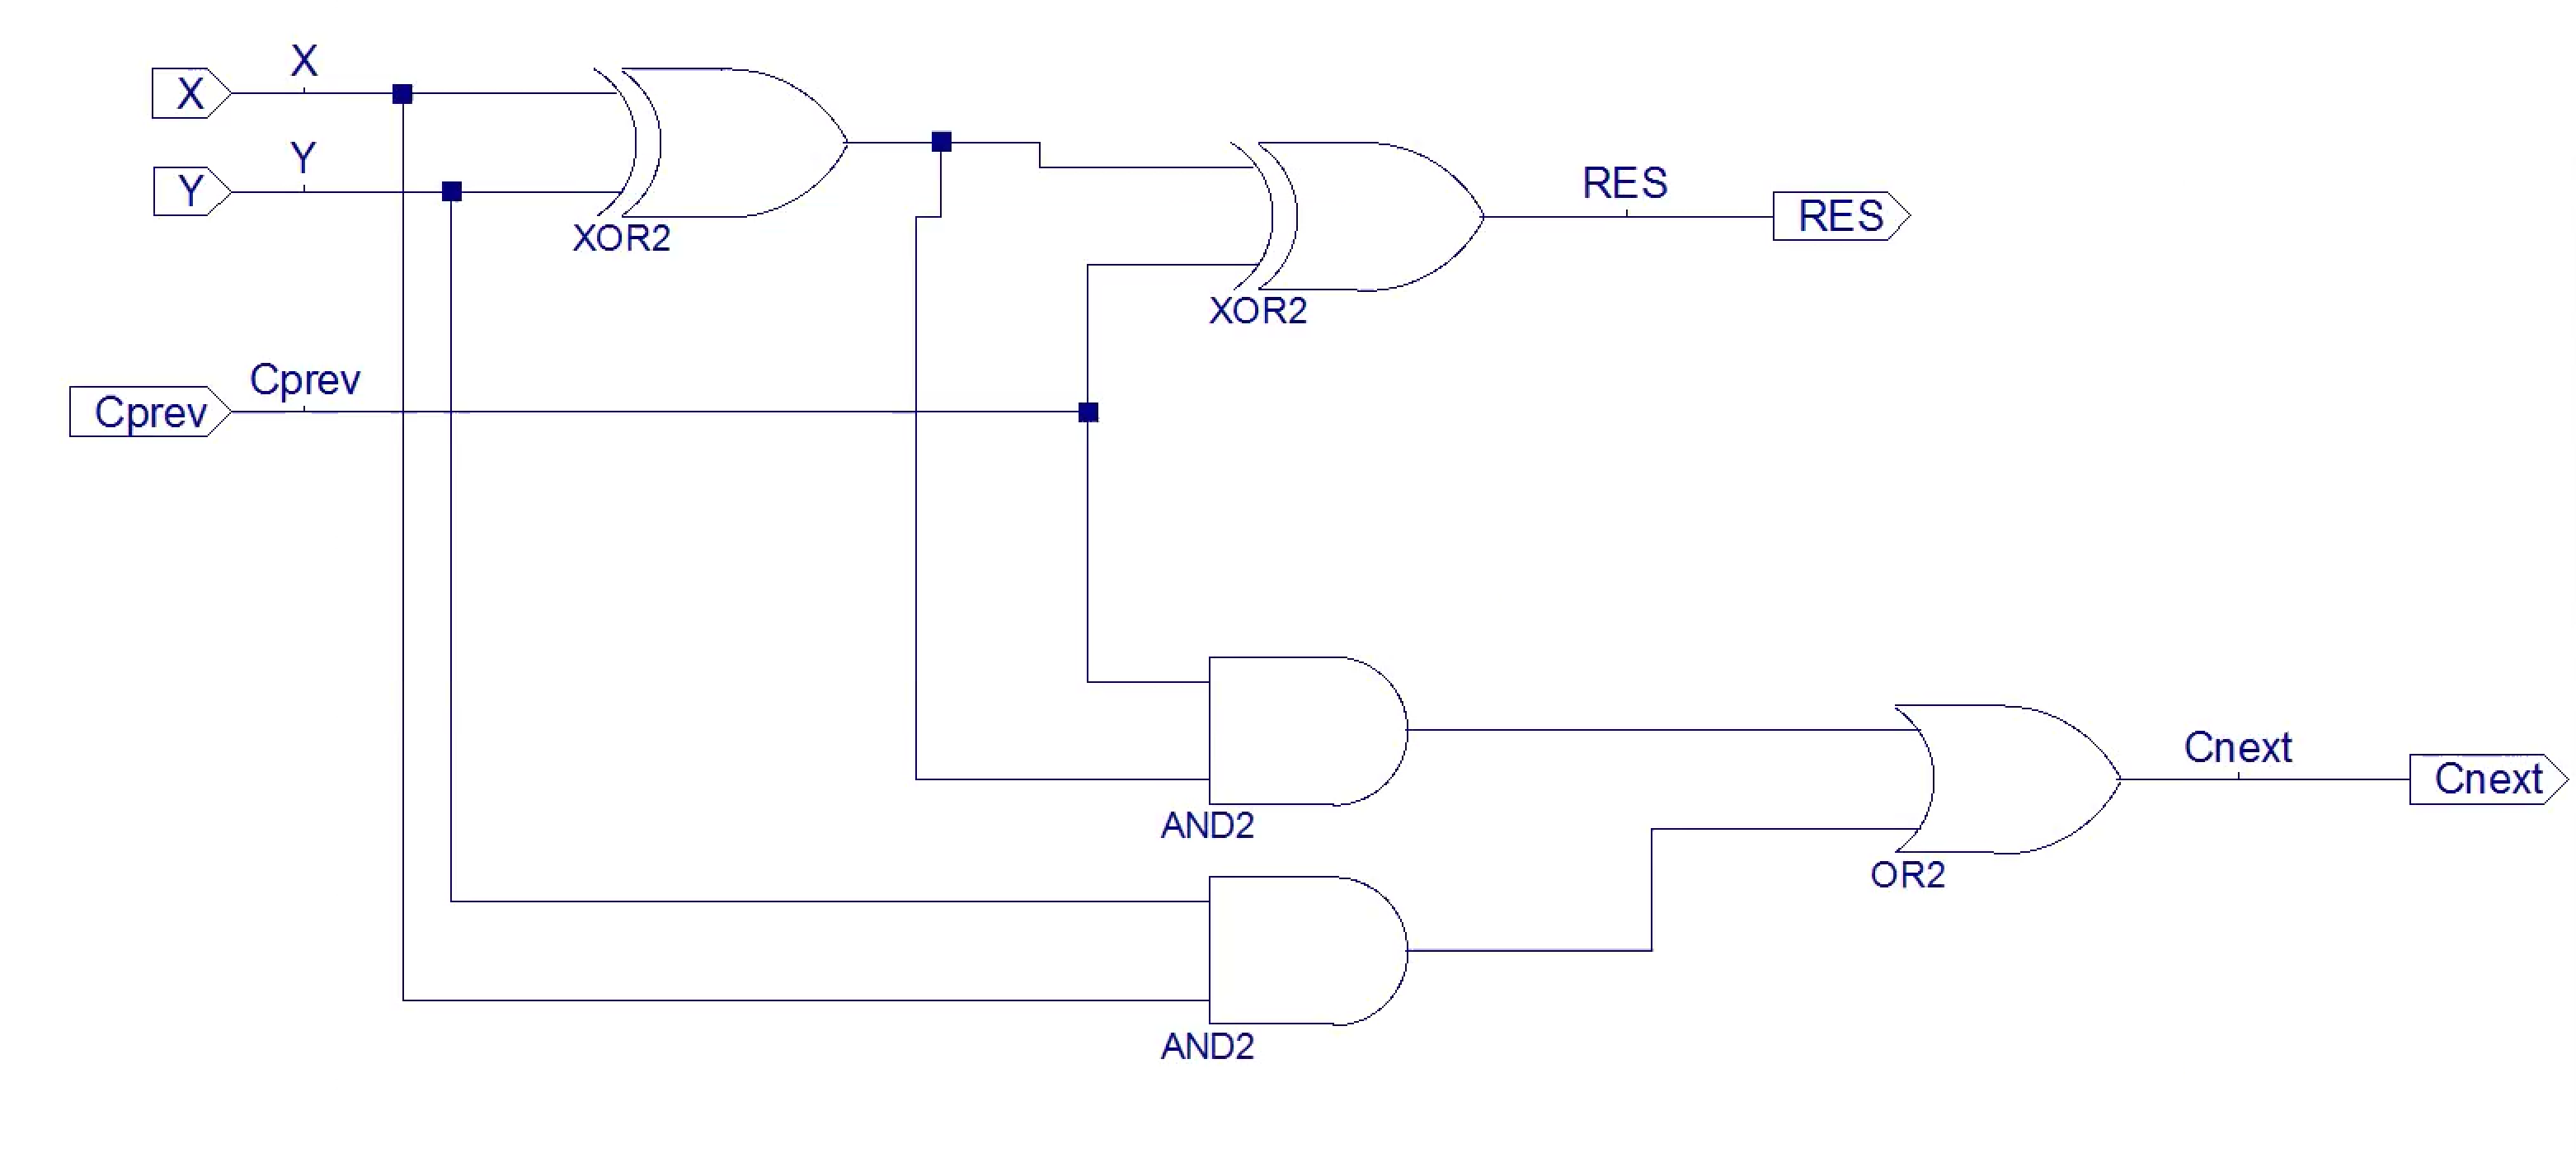
\includegraphics[scale=.3]{fa_sch.png}
%		\end{center}
		
		\begin{Verbatim}[frame=single, fontsize=\small]
`timescale 1ns/1ps

module fa_tbw_tb_0;
    reg Cprev = 1'b0;
    reg X = 1'b0;
    reg Y = 1'b0;
    wire Cnext;
    wire RES;

fa_sch UUT(
.Cprev(Cprev),
.X(X),
.Y(Y),
.Cnext(Cnext),
.RES(RES));

initial begin
#100;

//CASE 1
X=0;
Y=0;
Cprev=0;
#100;

//CASE 2
X=0;
Y=0;
Cprev=1;
#100;

//CASE 3
X=0;
Y=1;
Cprev=0;
#100;

//CASE 4
X=0;
Y=1;
Cprev=1;
#100;

//CASE 5
X=1;
Y=0;
Cprev=0;
#100;

//CASE 6
X=1;
Y=0;
Cprev=1;
#100;

//CASE 7
X=1;
Y=1;
Cprev=0;
#100;

//CASE 8
X=1;
Y=1;
Cprev=1;
#100;

end
	
endmodule
		\end{Verbatim}
		
		We then can add onto this by adding the ability to subtract and making it 8-bit, thus creating an 8-bit adder/subtractor
		
%		\begin{center}
%			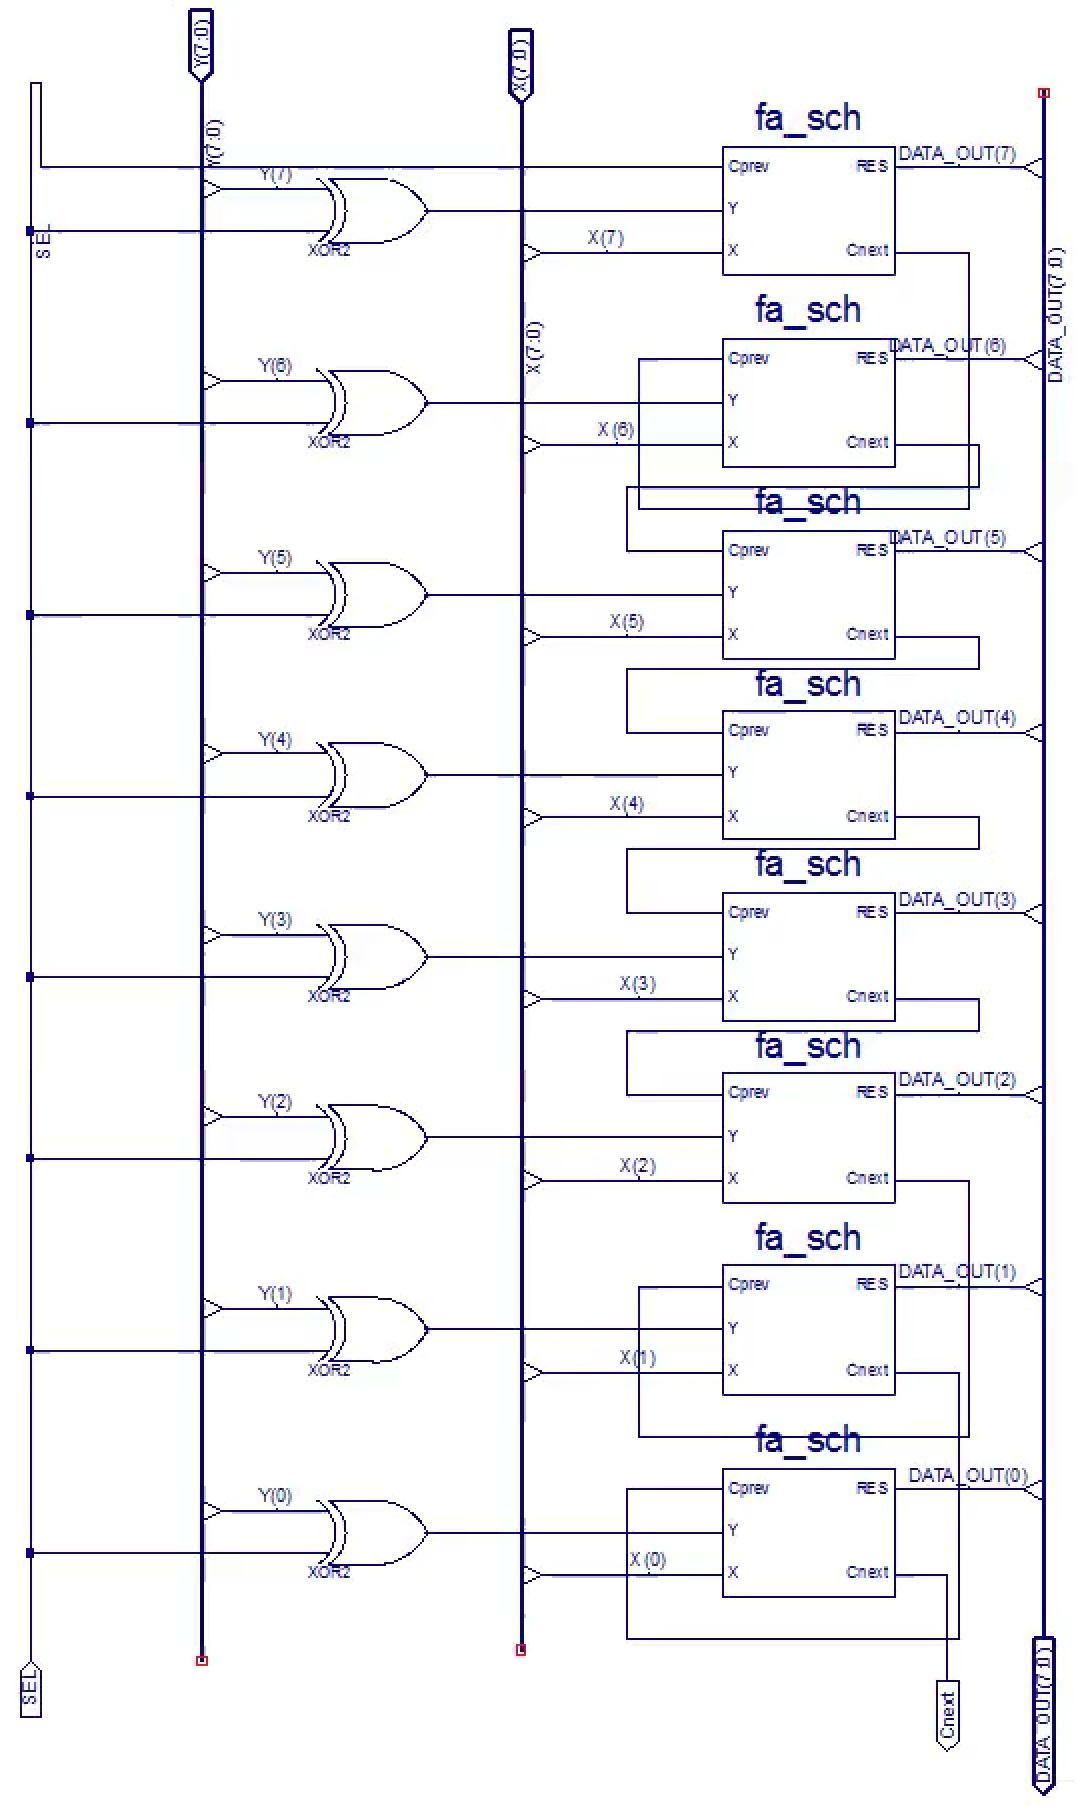
\includegraphics[scale=.5]{alu_sch.png}
%		\end{center}
		
		\begin{Verbatim}[frame=single, fontsize= \small]
`timescale 1ns / 1ps
//alu_sch_alu_sch_sch_tb
module alu_tbw_tb();

// Inputs
   reg [7:0] X = 8'b00000000;
   reg [7:0] Y = 8'b00000000;
   reg SEL = 1'b0;

// Output
   wire [7:0] DATA_OUT;
   wire Cnext;

// Instantiate the UUT
   alu_sch UUT (
		.X(X), 
		.DATA_OUT(DATA_OUT), 
		.Cnext(Cnext), 
		.Y(Y), 
		.SEL(SEL)
   );
// Initialize Inputs
initial begin     
#100;   //Wait 100ns for initial inputs to settle.      
for (i=0; i<max_count; i=i+1)           
	begin             
		{X,Y,SEL} = i;  //Cycle through all input combinations.             
		#100;   //Wait 100ns between new inputs.         
	end 
end 
endmodule
			
		\end{Verbatim}

		\newpage
	\subsection{Part 1}
		Next, we built a logic extender so that we can output logic operations to the full adder.
%		\begin{center}
%			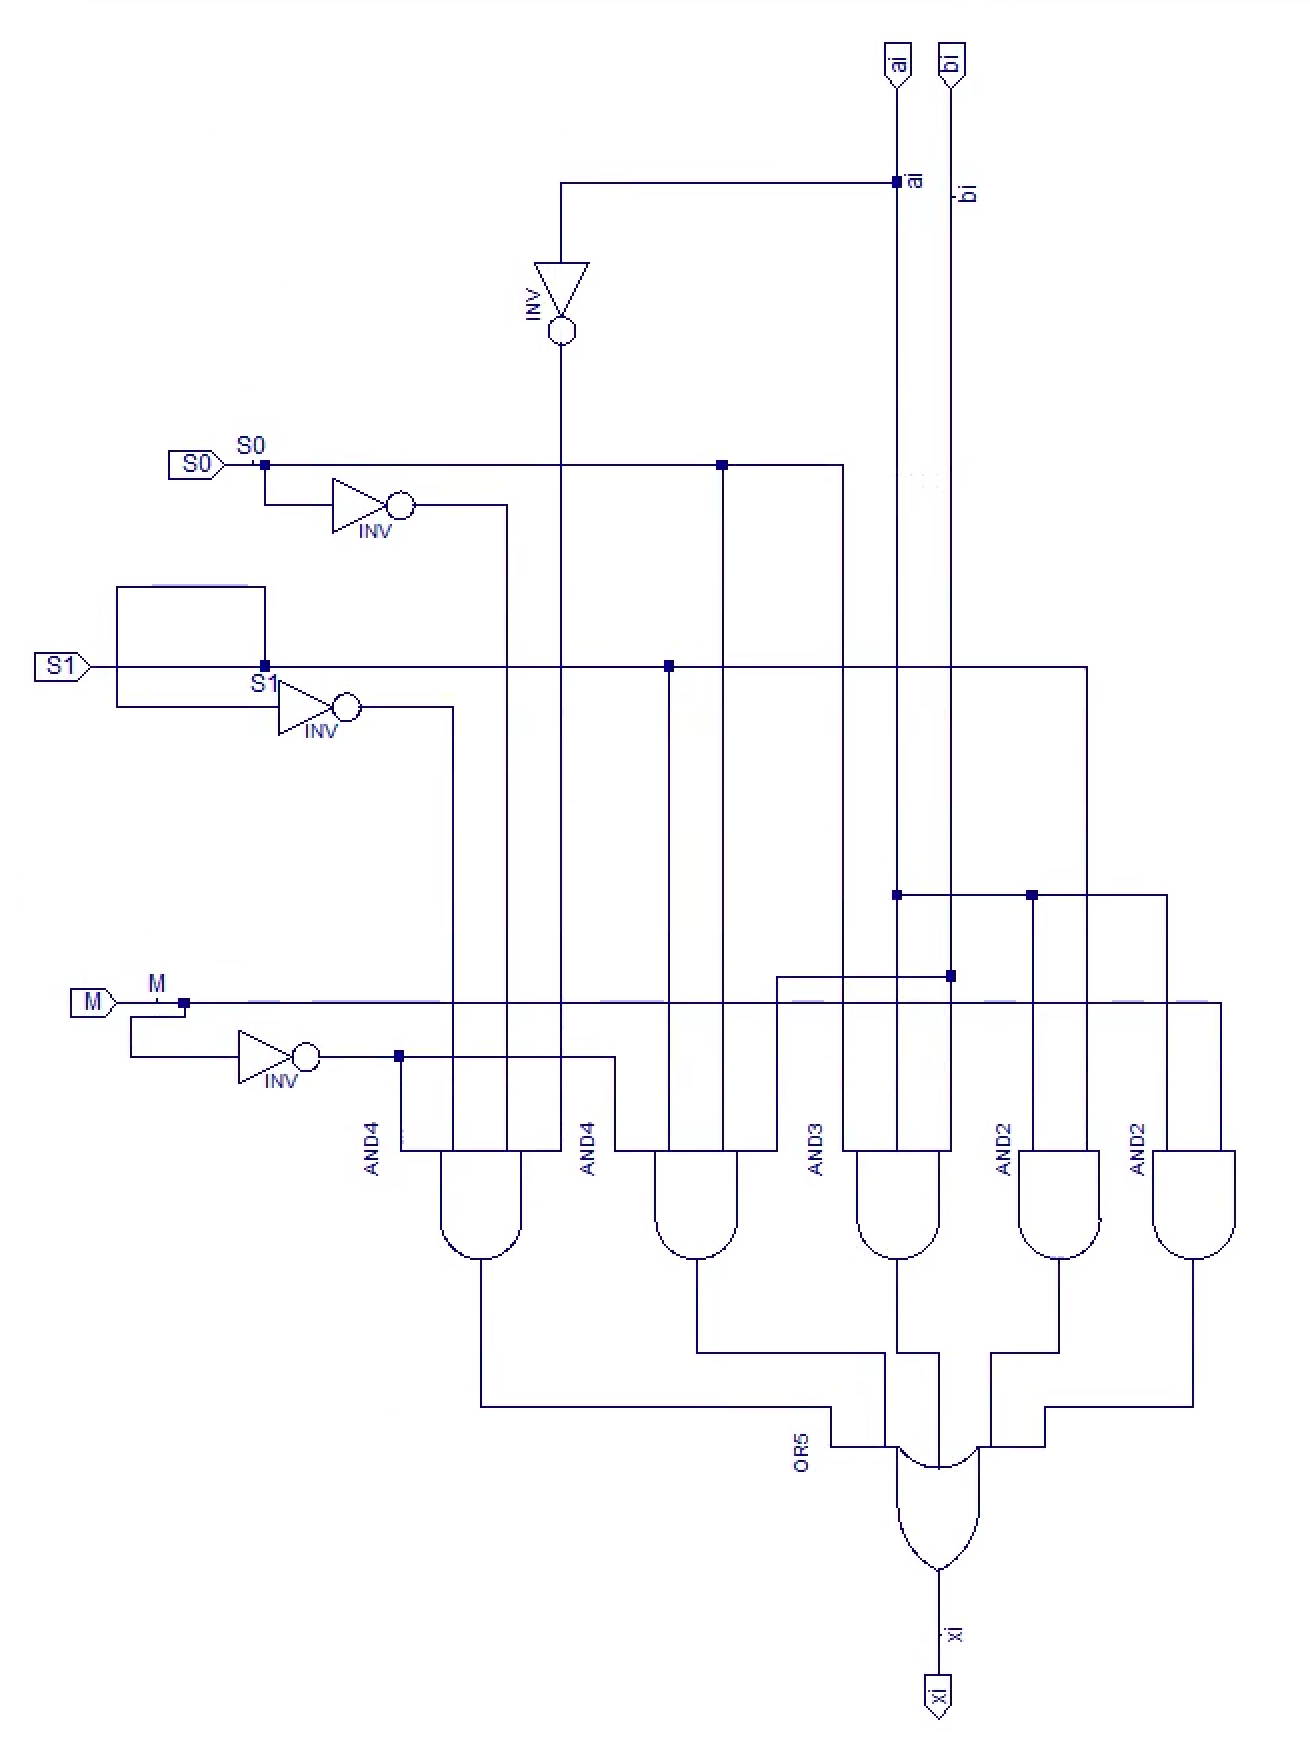
\includegraphics[scale=.5]{logic_ext_sch.png}
%		\end{center}
	
		\begin{Verbatim}[frame=single, fontsize= \small]
`timescale 1ns / 1ps

module logic_ext_tbw_tb_0;

// Inputs
   reg ai;
   reg bi;
   reg S0;
   reg S1;
   reg M;

// Output
   wire xi;
	
	integer i = 0; 
	parameter num_inputs = 5; 
	parameter max_count = (1<<num_inputs);

// Instantiate the UUT
   logic_ext UUT (
		.xi(xi), 
		.ai(ai), 
		.bi(bi), 
		.S0(S0), 
		.S1(S1), 
		.M(M)
   );
// Initialize Inputs
       initial begin
#100;
 for (i=0; i<max_count; i=i+1)
	begin {M,S1,S0,ai,bi} = i; 
	#100; 
	end
end
endmodule			
		\end{Verbatim}

	\newpage
	\subsection{Part 2}
		Similar to the Logic Extender, we will build an Arithmetic extender, which forwards arithmetic operations to the full adder rather than logic ones.
		
%		\begin{center}
%			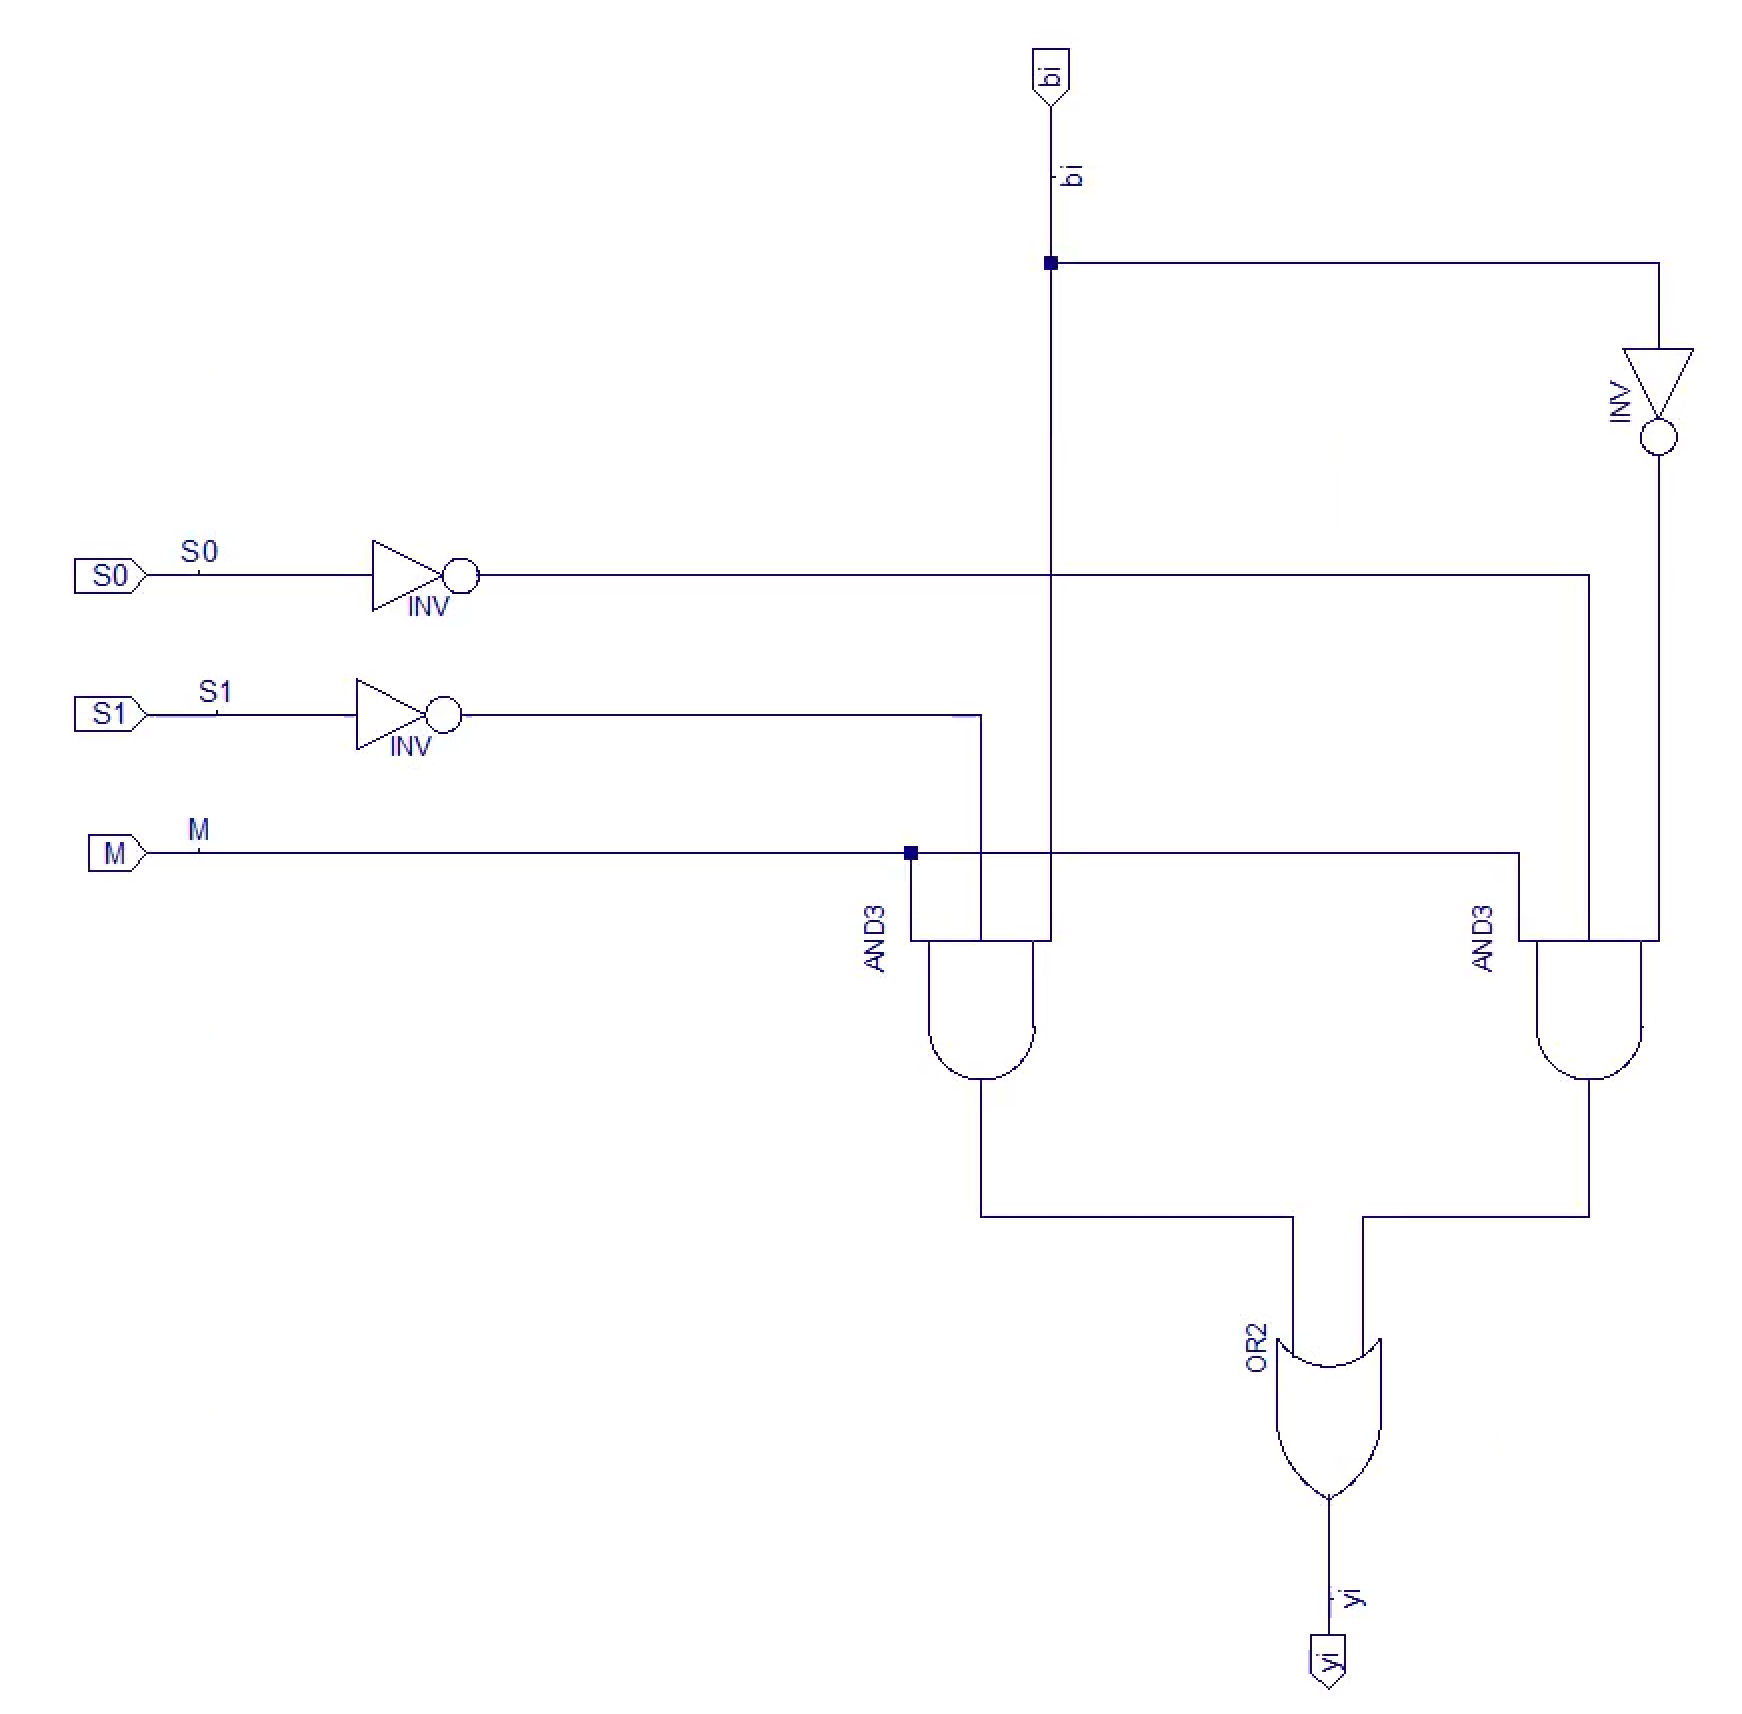
\includegraphics[scale=.5]{arith_ext_sch.png}
%		\end{center}

		\begin{Verbatim}[frame=single, fontsize=\small]
`timescale 1ns/1ps 
module arith_ext_tbw_tb_0;     
reg bi = 1'b0;     
reg M = 1'b0;     
reg S0 = 1'b0;     
reg S1 = 1'b0;     
wire yi;     
integer i = 0;    
parameter num_inputs = 4;     
parameter max_count = (1<<num_inputs); 
 
arith_ext UUT (     
.bi(bi),     
.M(M),     
.S0(S0),     
.S1(S1),     
.yi(yi)); 
  
initial begin     
#100;   //Wait 100ns for initial inputs to settle.      
for (i=0; i<max_count; i=i+1)           
	begin             
		{M,S1,S0,bi} = i;  //Cycle through all 4 input combinations.             
		#100;   //Wait 100ns between new inputs.         
	end 
end 
 
endmodule 
			
		\end{Verbatim}

	\subsection{Part 3}
		Now we can combine the previous parts into a working 4-bit ALU. In essence, we stack the Logic Extender and the Arithmetic Extender onto the Full Adder
%		\begin{center}
%			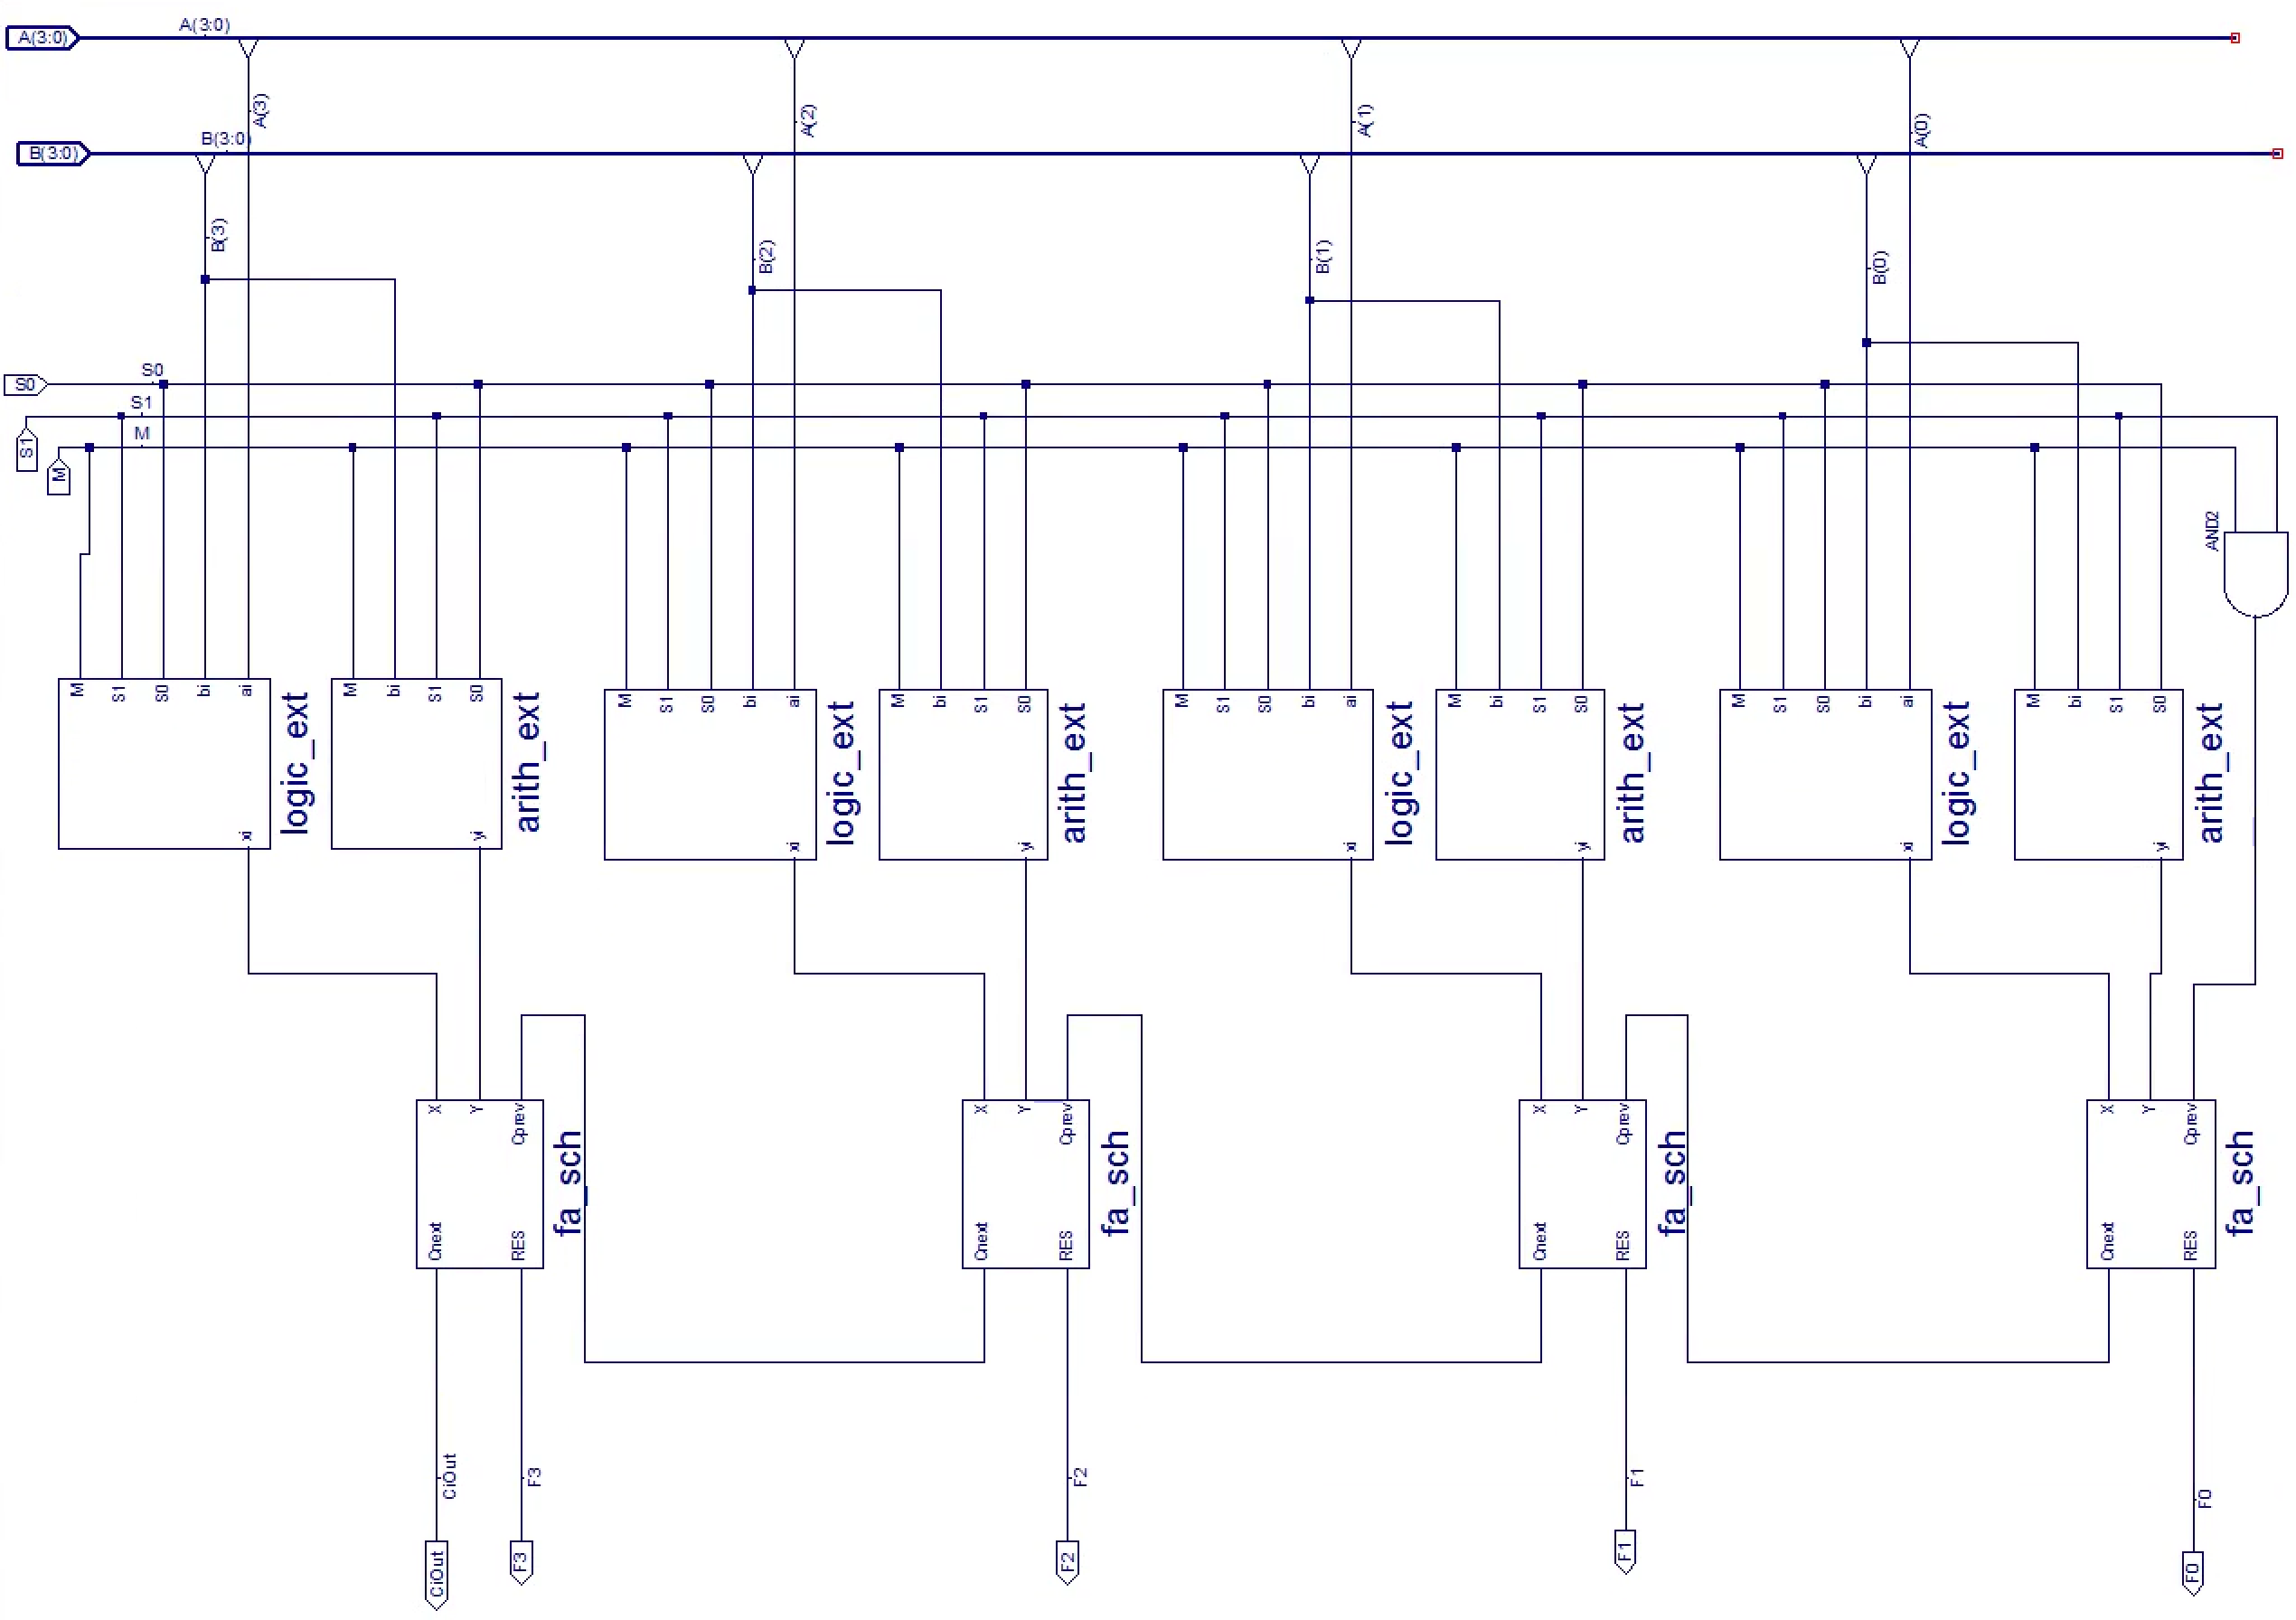
\includegraphics[scale=.3]{alu4bit_sch.png}
%		\end{center}
\newpage
		\begin{Verbatim}[frame=single, fontsize=\small]
`timescale 1ns / 1ps

module  alu4bit_tbw_tb_0;

// Inputs
   reg [3:0] A;
   reg [3:0] B;
   reg S0;
   reg S1;
   reg M;

// Output
   wire CiOut;
   wire F3;
   wire F2;
   wire F1;
   wire F0;

integer i =0;
parameter num_inputs =3;
parameter max_count = (1<<num_inputs);

// Instantiate the UUT
   alu4bit_sch UUT (
		.A(A), 
		.B(B), 
		.S0(S0), 
		.S1(S1), 
		.M(M), 
		.CiOut(CiOut), 
		.F3(F3), 
		.F2(F2), 
		.F1(F1), 
		.F0(F0)
   );
// Initialize Inputs

initial begin
#100;
for(i=0; i<max_count;i=i+1)
		begin
			{M,S1,S0}=i;
			A=4'b0101;
			B=4'b0100;
			#100;
		end
	#100;
	for(i=0; i<max_count;i=i+1)
		begin
			{M,S1,S0}=i;
			A=4'b1010;
			B=4'b0101;
			#100;
		end
	end
endmodule
			
		\end{Verbatim}
			
\section{Experimental Results}\vspace{-.7cm} \line(1,0){470}

%\begin{figure}[h]
%    \centering
%	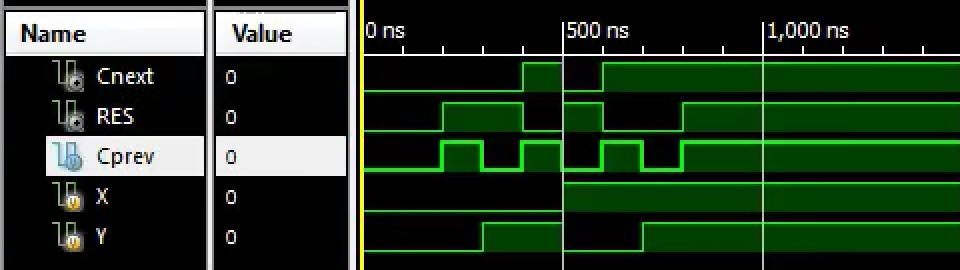
\includegraphics[scale=.7]{fa_tb_wave.png}
%	\caption{Waveform for the full adder schematic test bench. All test cases present for each value of X, Y, and Cprev, showing successful binary addition and carrying.}
%\end{figure}
%
%%\begin{figure}
%%	\includegraphics[scale=.7]{alu_tb_wave.png}
%%\end{figure}
%
%\begin{figure}[h]
%    \centering
%	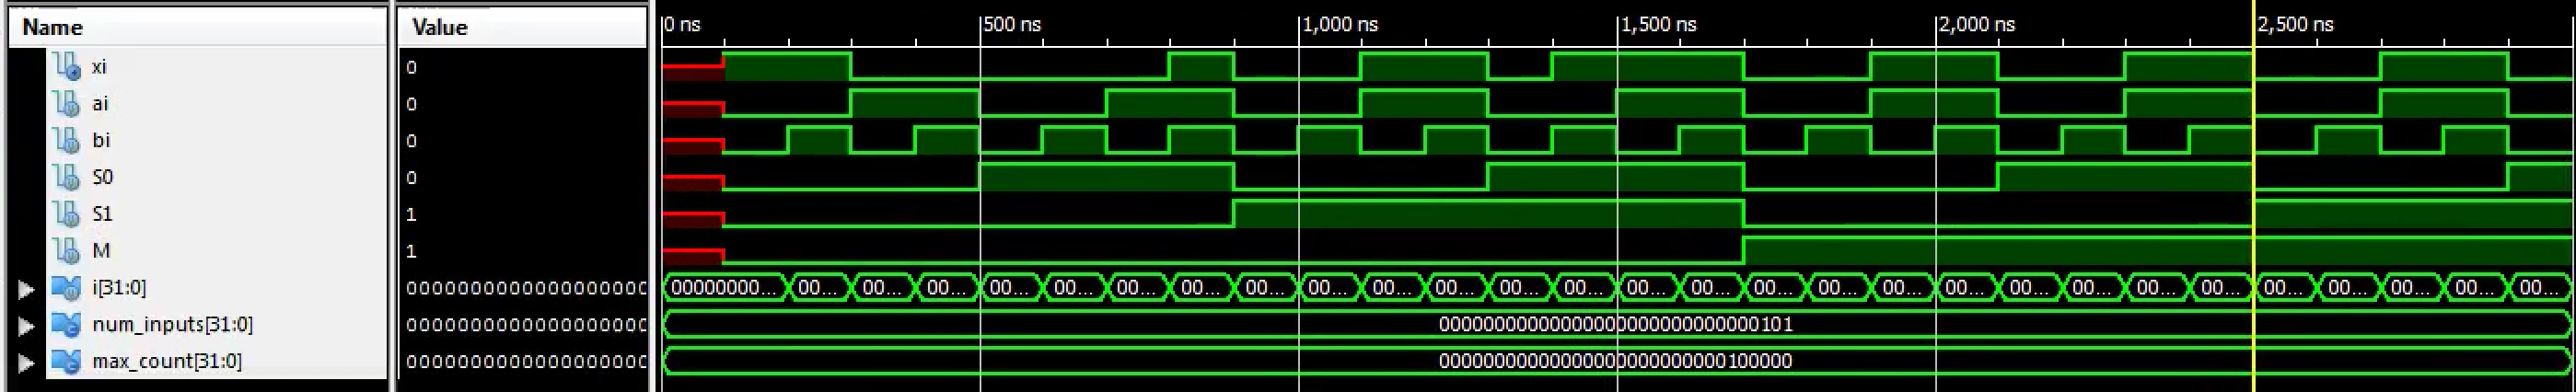
\includegraphics[scale=.33]{logic_ext_tb_wave}
%	\caption{Waveform for the logic extender schematic test bench. All test cases match that of the table given, successfully performing all required logic operations}
%\end{figure}
%
%\begin{figure}[h]
%    \centering
%	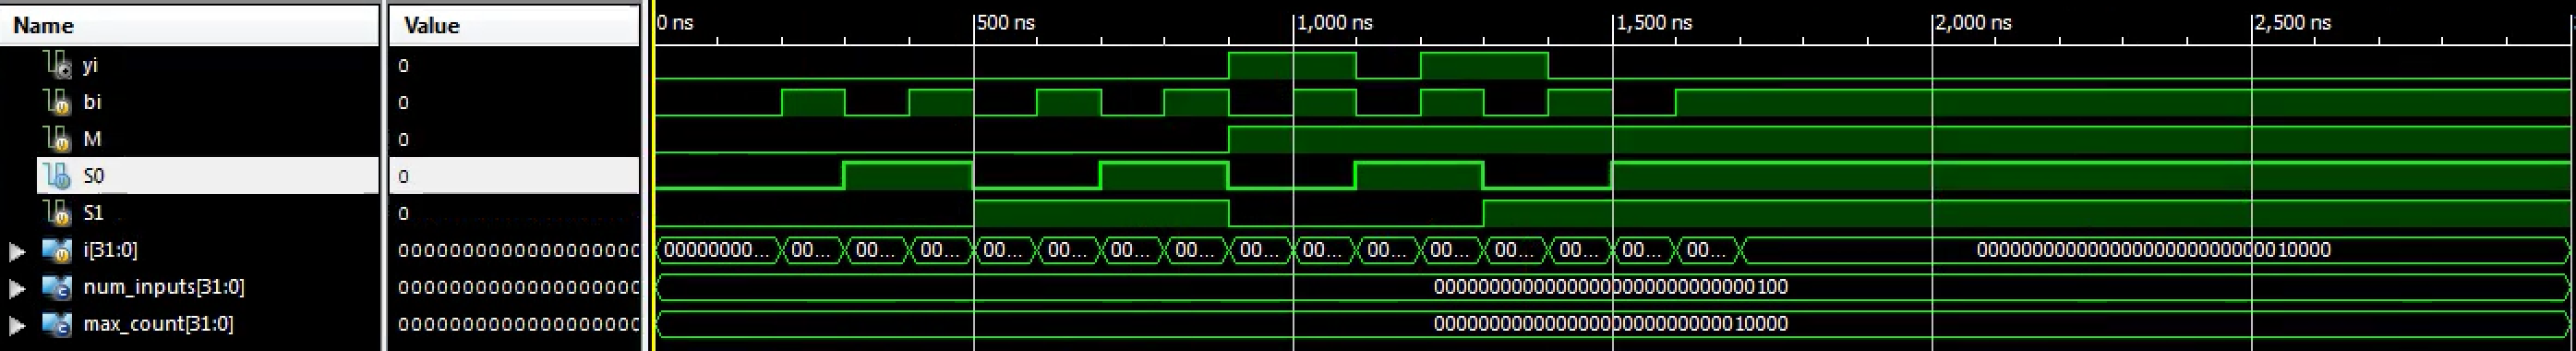
\includegraphics[scale=.33]{arith_ext_tb_wave.png}
%	\caption{Waveform for the arithmetic extender schematic test bench. All test cases match that of the table given, successfully performing all required arithmetic operations}
%\end{figure}
%
%\begin{figure}[h]
%    \centering
%	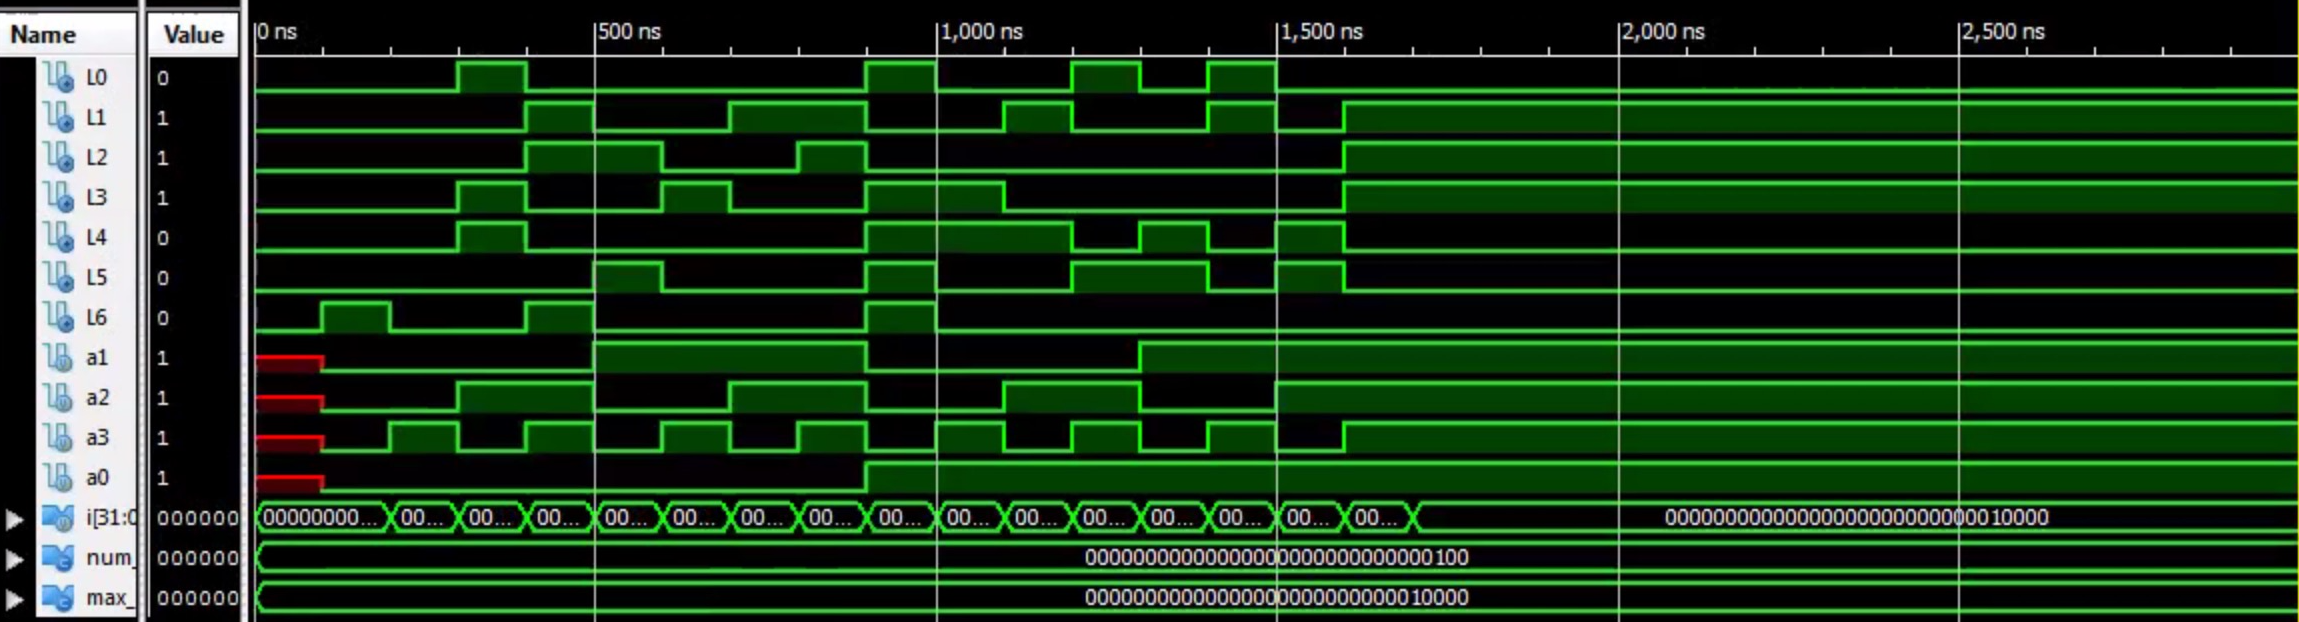
\includegraphics[scale=.2]{seven_segment_tb_wave.png}
%	\caption{Waveform for the seven segment display driver, showing all possible combinations for the 4-bit binary input, and corresponding outputs.}
%\end{figure}
%
%\begin{figure}[ht]
%    \centering
%	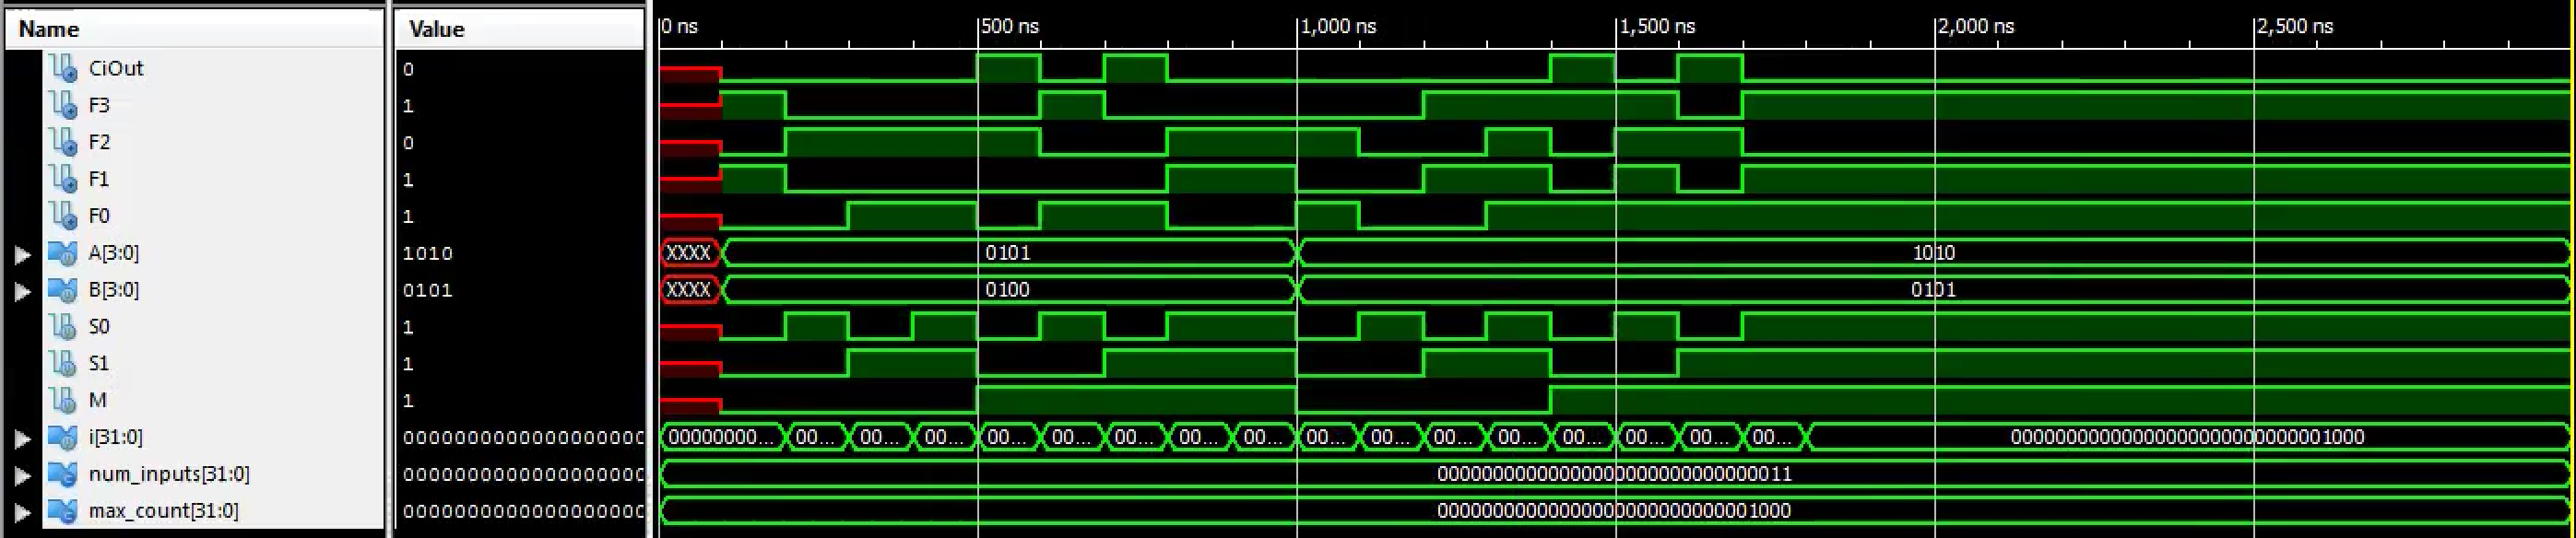
\includegraphics[scale=.33]{alu4bit_tb_wave.png}
%	\caption{Waveform for the 4-bit ALU, testing again each possible input combination of S0, S1, and M.}
%\end{figure}

	\newpage
\section{Significance} \vspace{-.7cm} \line(1,0){470}
	\paragraph{}
		This lab was the first comprehensive use of the Xilinx GUI schematic creator, and using it to create several modules that would eventually create a full project, and eventually exist on the board. While this did feel like a full, independent project of its own, in reality it is just the first piece of a much bigger puzzle that is a usable CPU. With the knowledge gained in this lab, piecing the parts together makes much more sense now. 

 \section{Comments/Suggestions}\vspace{-.7cm} \line(1,0){470}
 	\paragraph{}
		Everything was rather straightforward, although it was relatively quite a bit of work. In the future, it may be best to assign a portion of the lab as prelab, so that it could be more spread out.
		
\end{document}


